\documentclass[english]{article}
\usepackage[T1]{fontenc}
\usepackage[utf8]{luainputenc}
\usepackage{graphicx}
\usepackage{babel}
\title{\textbf{Data acquisition system for the Glass RPC Semi Digital HCAL}}
\author{Laurent Mirabito\\
		Christophe Combaret\\
		}
\date{}
\begin{document}

\maketitle

\section{Introduction}

The Glass RPC semi digital hadronic calorimeter prototype was described in \cite{RPC-paper}. This paper will describe the architecture of the readout. The schematic of the acquistion can be seen on figure \ref{daq-schematic}


\begin{figure}[htp]
\centering
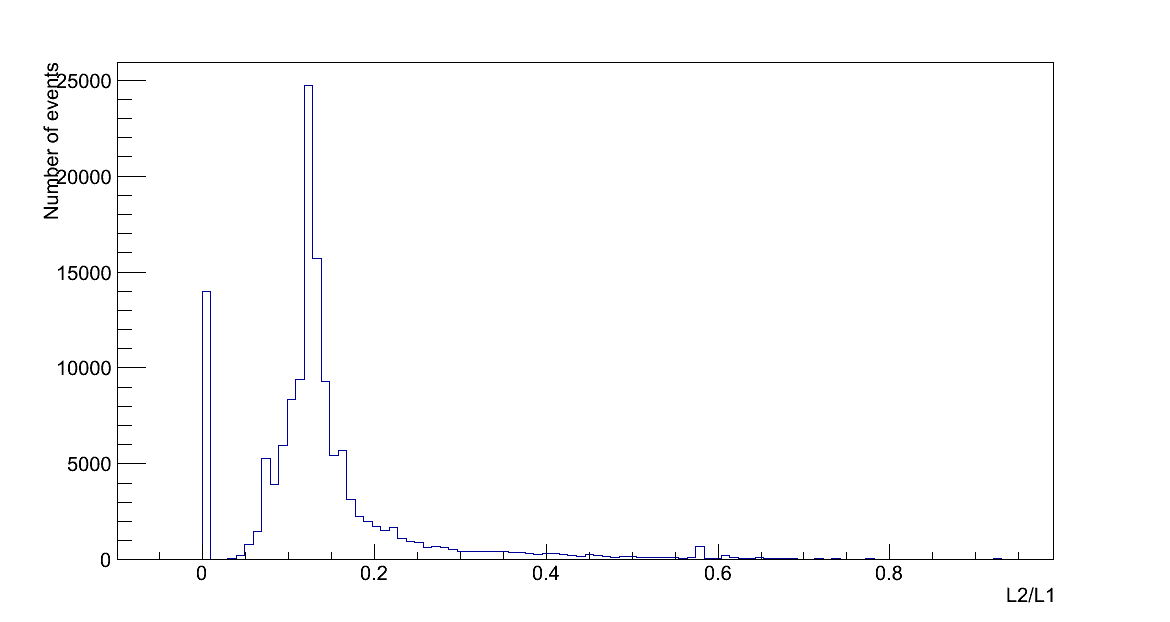
\includegraphics[scale=1.00]{/home/odroid/MesNotes/SDHCALNote/Hits_Weight_track.png}
\caption{Schematic of the SDHCAL readout}
\label{daq-schematic}
\end{figure}

\end{document}
